\documentclass[11pt]{article}
\usepackage[pdftex]{graphicx, color}
\usepackage{listings}

\usepackage{tikz}
\usetikzlibrary{automata,positioning}

\headheight 8pt \headsep 20pt \footskip 30pt
\textheight 9in \textwidth 6.5in
\oddsidemargin 0in \evensidemargin 0in
\topmargin -.35in

\lstset{basicstyle=\small\ttfamily,breaklines=true}

\begin{document}
\begin{center}
\LARGE CS143 Spring 2020 - Written Assignment 1 \\
\large Due Thursday, April 23, 2016 at 11:59 PM
\end{center}

This assignment covers regular languages, finite automata and lexical analysis. You may discuss this assignment with other students and work on the problems together. However, your write-up should be your own individual work, and you should indicate in your submission who you worked with, if applicable. Assignments can be submitted electronically throught Gradescope as a PDF by 11:59 PM PDT. A \LaTeX \ template for writing your solutions is available on the course website. There is a post on Piazza describing how to create the finite automata diagrams.

\begin{enumerate}
  % Problem 1
  \item Write regular expressions for the following languages over the alphabet $\Sigma = \{0, 1\}$:
  \begin{enumerate}
    \item The set of all strings where no two consecutive characters are the same.
    \item The set of all strings representing a binary number that is a power of 2. Allow for leading zeros e.g. 001000.
    \item The set of all strings containing at least one of 1110 or 1011.
  \end{enumerate}
  
  % Problem 2
  % See Piazza post for how to generate DFAs
  \item Draw the DFAs for each of the languages from Question 1.
  
  % Problem 3
  \item Using the techniques covered in class, transform the following NFAs with $\epsilon$-transitions over the given alphabet $\Sigma$ into DFAs. Note that a DFA must have a transition defined for every state and symbol pair, whereas a NFA need not. You must take this fact into account for your transformations. Hint: Is there a subset of states the NFA transitions to when fed a symbol for which the set of current states has no explicit transition?
  
  \begin{enumerate}
    \item $\Sigma$ = $\{a, b, c\}$ \\ 
\begin{center}
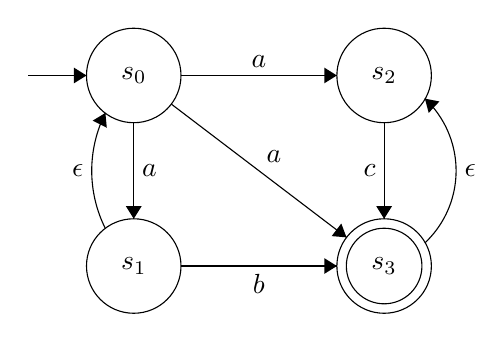
\begin{tikzpicture}[scale=0.2]
\tikzstyle{every node}+=[inner sep=0pt]
\draw [black] (14.8,-11.1) circle (3);
\draw (14.8,-11.1) node {$s_0$};
\draw [black] (30.7,-11.1) circle (3);
\draw (30.7,-11.1) node {$s_2$};
\draw [black] (14.8,-23.2) circle (3);
\draw (14.8,-23.2) node {$s_1$};
\draw [black] (30.7,-23.2) circle (3);
\draw (30.7,-23.2) node {$s_3$};
\draw [black] (30.7,-23.2) circle (2.4);
\draw [black] (8.1,-11.1) -- (11.8,-11.1);
\fill [black] (11.8,-11.1) -- (11,-10.6) -- (11,-11.6);
\draw [black] (17.8,-11.1) -- (27.7,-11.1);
\fill [black] (27.7,-11.1) -- (26.9,-10.6) -- (26.9,-11.6);
\draw (22.75,-10.6) node [above] {$a$};
\draw [black] (14.8,-14.1) -- (14.8,-20.2);
\fill [black] (14.8,-20.2) -- (15.3,-19.4) -- (14.3,-19.4);
\draw (15.3,-17.15) node [right] {$a$};
\draw [black] (17.19,-12.92) -- (28.31,-21.38);
\fill [black] (28.31,-21.38) -- (27.98,-20.5) -- (27.37,-21.3);
\draw (23.7,-16.65) node [above] {$a$};
\draw [black] (30.7,-14.1) -- (30.7,-20.2);
\fill [black] (30.7,-20.2) -- (31.2,-19.4) -- (30.2,-19.4);
\draw (30.2,-17.15) node [left] {$c$};
\draw [black] (17.8,-23.2) -- (27.7,-23.2);
\fill [black] (27.7,-23.2) -- (26.9,-22.7) -- (26.9,-23.7);
\draw (22.75,-23.7) node [below] {$b$};
\draw [black] (13,-20.821) arc (-153.38582:-206.61418:8.194);
\fill [black] (13,-13.48) -- (12.19,-13.97) -- (13.09,-14.42);
\draw (11.63,-17.15) node [left] {$\epsilon$};
\draw [black] (33.285,-12.565) arc (46.79805:-46.79805:6.29);
\fill [black] (33.29,-12.57) -- (33.53,-13.48) -- (34.21,-12.75);
\draw (35.77,-17.15) node [right] {$\epsilon$};
\end{tikzpicture}
\end{center}
\item $\Sigma$ = $\{a, b, c\}$ \\ 
\begin{center}
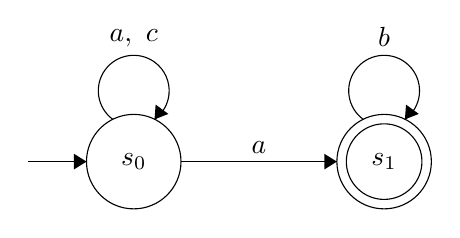
\begin{tikzpicture}[scale=0.2]
\tikzstyle{every node}+=[inner sep=0pt]
\draw [black] (14.8,-11.1) circle (3);
\draw (14.8,-11.1) node {$s_0$};
\draw [black] (30.7,-11.1) circle (3);
\draw (30.7,-11.1) node {$s_1$};
\draw [black] (30.7,-11.1) circle (2.4);
\draw [black] (29.377,-8.42) arc (234:-54:2.25);
\draw (30.7,-3.85) node [above] {$b$};
\fill [black] (32.02,-8.42) -- (32.9,-8.07) -- (32.09,-7.48);
\draw [black] (17.8,-11.1) -- (27.7,-11.1);
\fill [black] (27.7,-11.1) -- (26.9,-10.6) -- (26.9,-11.6);
\draw (22.75,-10.6) node [above] {$a$};
\draw [black] (13.477,-8.42) arc (234:-54:2.25);
\draw (14.8,-3.85) node [above] {$a,\mbox{ }c$};
\fill [black] (16.12,-8.42) -- (17,-8.07) -- (16.19,-7.48);
\draw [black] (8.1,-11.1) -- (11.8,-11.1);
\fill [black] (11.8,-11.1) -- (11,-10.6) -- (11,-11.6);
\end{tikzpicture}
\end{center}
\newpage
\item $\Sigma$ = $\{a, b\}$ \\ 
\begin{center}
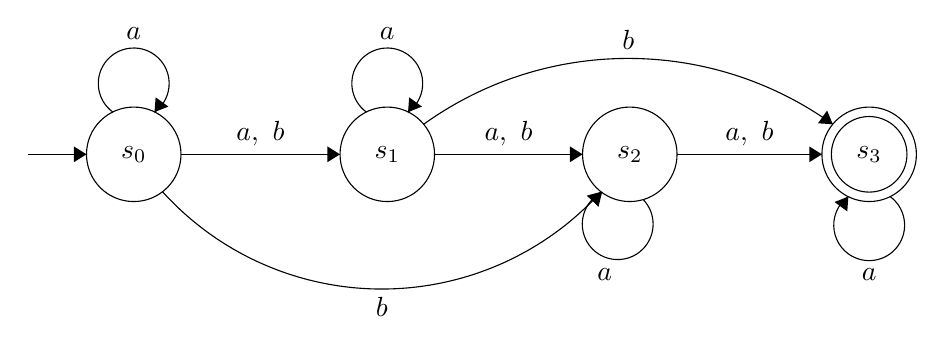
\begin{tikzpicture}[scale=0.2]
\tikzstyle{every node}+=[inner sep=0pt]
\draw [black] (14.6,-10.9) circle (3);
\draw (14.6,-10.9) node {$s_0$};
\draw [black] (30.7,-10.9) circle (3);
\draw (30.7,-10.9) node {$s_1$};
\draw [black] (46.1,-10.9) circle (3);
\draw (46.1,-10.9) node {$s_2$};
\draw [black] (61.3,-10.9) circle (3);
\draw (61.3,-10.9) node {$s_3$};
\draw [black] (61.3,-10.9) circle (2.4);
\draw [black] (7.9,-10.9) -- (11.6,-10.9);
\fill [black] (11.6,-10.9) -- (10.8,-10.4) -- (10.8,-11.4);
\draw [black] (13.277,-8.22) arc (234:-54:2.25);
\draw (14.6,-3.65) node [above] {$a$};
\fill [black] (15.92,-8.22) -- (16.8,-7.87) -- (15.99,-7.28);
\draw [black] (17.6,-10.9) -- (27.7,-10.9);
\fill [black] (27.7,-10.9) -- (26.9,-10.4) -- (26.9,-11.4);
\draw (22.65,-10.4) node [above] {$a,\mbox{ }b$};
\draw [black] (44.273,-13.276) arc (-42.13785:-137.86215:18.776);
\fill [black] (44.27,-13.28) -- (43.37,-13.53) -- (44.11,-14.2);
\draw (30.35,-19.95) node [below] {$b$};
\draw [black] (29.377,-8.22) arc (234:-54:2.25);
\draw (30.7,-3.65) node [above] {$a$};
\fill [black] (32.02,-8.22) -- (32.9,-7.87) -- (32.09,-7.28);
\draw [black] (33.7,-10.9) -- (43.1,-10.9);
\fill [black] (43.1,-10.9) -- (42.3,-10.4) -- (42.3,-11.4);
\draw (38.4,-10.4) node [above] {$a,\mbox{ }b$};
\draw [black] (46.945,-13.766) arc (44.15497:-243.84503:2.25);
\draw (44.51,-18.14) node [below] {$a$};
\fill [black] (44.34,-13.31) -- (43.42,-13.51) -- (44.11,-14.23);
\draw [black] (33.011,-8.991) arc (125.68886:54.31114:22.264);
\fill [black] (58.99,-8.99) -- (58.63,-8.12) -- (58.05,-8.93);
\draw (46,-4.31) node [above] {$b$};
\draw [black] (49.1,-10.9) -- (58.3,-10.9);
\fill [black] (58.3,-10.9) -- (57.5,-10.4) -- (57.5,-11.4);
\draw (53.7,-10.4) node [above] {$a,\mbox{ }b$};
\draw [black] (62.623,-13.58) arc (54:-234:2.25);
\draw (61.3,-18.15) node [below] {$a$};
\fill [black] (59.98,-13.58) -- (59.1,-13.93) -- (59.91,-14.52);
\end{tikzpicture}
\end{center}
  \end{enumerate}  

  % Problem 4
    \item Let $L$ be the language over $\Sigma$ = ${a,b,c}$ where the following holds: $w$ is in $L$ if at most one character has more than one occurrence in w.   \\ \\ 
Examples of Strings in $L$: a, baaaaaac, $\epsilon$ \\  
Examples of Strings \textbf{not} in $L$: ccbb, abcab\\ \\  
Draw an NFA for $L$.
  
  % Problem 5
  \item Consider the following tokens and their associated regular expressions, given as a \textbf{flex} scanner specification:
  
  \begin{lstlisting}
    %%
    (01|10)                 printf("snake")
    0(01)*1                 printf("badger")
    (1010*1|0101*0)         printf("mushroom")
  \end{lstlisting}
  
  Give an input to this scanner such that the output string is $\tt (badger^{\rm 11}  mushroom^{\rm 2})^{\rm 4}\ snake^{\rm 3}$, where $\tt A^i$ denotes {\tt A} repeated {\tt i} times.   (And, of course, the parentheses are not part of the output.)  You may use similar shorthand notation in your answer.
  
  % Problem 6
  \item Recall from the lecture that, when using regular expressions to scan an input, we resolve conflicts by taking the largest possible match at any point. That is, if we have the following \textbf{flex} scanner specification:
  
  \begin{lstlisting}
    %%
    do                      { return T_Do; }
    [A-Za-z_][A-Za-z0-9_]*  { return T_Identifier; }
  \end{lstlisting} 
  
  and we see the input string ``dot'', we will match the second rule and emit $\tt T\_Identifier$ for the whole string, not $\tt T\_Do$.
  
  However, it is possible to have a set of regular expressions for which we can tokenize a particular string, but for which taking the largest possible match will fail to break the input into tokens. Give an example of a set of regular expressions and an input string such that: a) the string can be broken into substrings, where each substring matches one of the regular expressions, b) our usual lexer algorithm, taking the largest match at every step, will fail to break the string in a way in which each piece matches one of the regular expressions. Explain how the string can be tokenized and why taking the largest match won't work in this case.

\end{enumerate}
\end{document}
